% easychair.tex,v 3.5 2017/03/15

\documentclass{easychair}
%\documentclass[EPiC]{easychair}
%\documentclass[EPiCempty]{easychair}
%\documentclass[debug]{easychair}
%\documentclass[verbose]{easychair}
%\documentclass[notimes]{easychair}
%\documentclass[withtimes]{easychair}
%\documentclass[a4paper]{easychair}
%\documentclass[letterpaper]{easychair}

\usepackage{doc}
\usepackage[utf8]{inputenc}

\usepackage{tikz}
\usetikzlibrary{positioning,fit,shapes,arrows.meta}

\usepackage{minted}

\usepackage{todonotes}
\newcommand{\as}[1]{\todo[color=blue!30,caption={}]{#1}}
\newcommand{\asi}[1]{\todo[color=blue!30,inline]{#1}}
% use this if you have a long article and want to create an index
% \usepackage{makeidx}

% In order to save space or manage large tables or figures in a
% landcape-like text, you can use the rotating and pdflscape
% packages. Uncomment the desired from the below.
%
% \usepackage{rotating}
% \usepackage{pdflscape}

%% Front Matter
%%
% Regular title as in the article class.
%
\title{MLExplain}

% Authors are joined by \and. Their affiliations are given by \inst, which indexes
% into the list defined using \institute
%
\author{
  Kévin Le Bon\inst{1}
  \and
  Alan Schmitt\inst{1}
}

% Institutes for affiliations are also joined by \and,
\institute{
  Inria
 }

%  \authorrunning{} has to be set for the shorter version of the authors' names;
% otherwise a warning will be rendered in the running heads. When processed by
% EasyChair, this command is mandatory: a document without \authorrunning
% will be rejected by EasyChair

\authorrunning{Le Bon and Schmitt}

% \titlerunning{} has to be set to either the main title or its shorter
% version for the running heads. When processed by
% EasyChair, this command is mandatory: a document without \titlerunning
% will be rejected by EasyChair
\titlerunning{MLExplain}

\begin{document}

\maketitle

\begin{abstract}
MLExplain est un interpréteur visuel pas-à-pas de OCaml permettant
d'inspecter non seulement l'état du programme exécuté mais également
l'état de l'interpréteur.
\end{abstract}

\section{Introduction}

La sémantique d'un langage de programmation peut être très complexe. Lorsque
qu'un langage ne possède pas de spécification, la sémantique correspond alors
aux implémentations (interpréteurs et compilateurs) du langage. Mais même en
présence d'une spécification, il peut être difficile de comprendre pourquoi
l'exécution d'un programme particulier donne un certain résultat.

Le projet JSExplain\footnote{\url{https://github.com/jscert/jsexplain}} a pour
objectif de décrire l'exécution d'un programme JavaScript en montrant toutes les
étapes d'un interpréteur très proche de la spécification de JavaScript. Ce
papier montre comment nous avons adapté JSExplain au langage OCaml.

À la différence de JavaScript, OCaml ne possède pas de spécification. En
revanche, l'exécution de code OCaml est particulièrement simple car le nombre de
constructions manipulées est très réduit. Nous avons ainsi écrit un interpréteur
pour l'arbre de syntaxe abstrait (AST) typé de OCaml. Cet AST reste proche du
code source, et s'appuyer sur la version typée permet entre autres d'avoir accès
aux noms complètement résolus, ce qui est très utile pour la résolution
d'inclusion de modules et de signatures. La sémantique que nous proposons est
plus haut niveau que celle décrite par la machine abstraite ZINC
\cite{Leroy-ZINC}, qui se situe au niveau d'un code objet produit par un
compilateur. 

Pas besoin de parler de GC.

Donner le langage d'entrée (quelle tête à l'AST)

\begin{itemize}
\item Présentation de JSExplain
  \begin{itemize}
  \item Son fonctionnement
    \begin{itemize}
    \item Ce qu'il fait et comment il s'y prend
    \end{itemize}
  \item sous langage OCaml pris en entrée
    \begin{itemize}
    \item mise en évidence des limites du compilateur OCaml vers JS
    \end{itemize}
  \item sous langage JavaScript généré
  \item compilateur et annotations
    \begin{itemize}
    \item tranformation des types OCaml en objets JS grâce aux annotations
    \item traces
    \end{itemize}
  \end{itemize}
\item Présentation de MLExplain
  \begin{itemize}
  \item le problème du parser, expliquer comment on s'en sort
    \begin{itemize}
    \item utilisation de js\_of\_ocaml comme 2e compilateur
    \end{itemize}
  \item contraster la taille du code de l'interpréteur ML vs JS
    \begin{itemize}
    \item OCaml ayant une sémantique très simple et un nombre de features limité (sans compter l'objet et encore) contrairement à Javascript, on montre que ça se reflète très clairement dans la taille et la complexité du code des interpréteurs
    \end{itemize}
  \item capture d'écran
    \begin{itemize}
    \item page web de MLExplain avec explication des différentes parties qui la composent
    \end{itemize}
  \item le problème de la bibliothèque standard
    \begin{itemize}
    \item problème de tout code externe à celui écrit directement à la textearea de la page web de MLExplain d'ailleurs
    \end{itemize}
  \item Résultats/Conclusion
  \end{itemize}
\end{itemize}

\section{L'interpréteur visuel JSExplain}

Un interpréteur est un programme qui prend du code écrit dans un langage 
spécifique en entrée, et l'exécute. Dans ce but, l'interpréteur effectue un 
certain nombre d'analyses dont les plus communes : l'analyse lexicale, 
l'analyse syntaxique, le typage.

Nous appelons \emph{interpréteur visuel} un interpréteur qui permet d'afficher
l'état du programme, position dans le source et valeurs des variables locales,
au fur et à mesure de son exécution, ainsi que l'état de l'interpréteur.
JSExplain\footnote{https://github.com/jscert/jsexplain} est un interpréteur
visuel pour le langage JavaScript. Le but de cet outil est de permettre de mieux
comprendre la sémantique du JavaScript. Pour ce faire, l'interface met en
évidence l'expression du programme source en cours d'évaluation ainsi que
l'instruction de l'interpréteur exécutée.

\subsection{Architecture de JSExplain}

\begin{figure*}
  \centering
  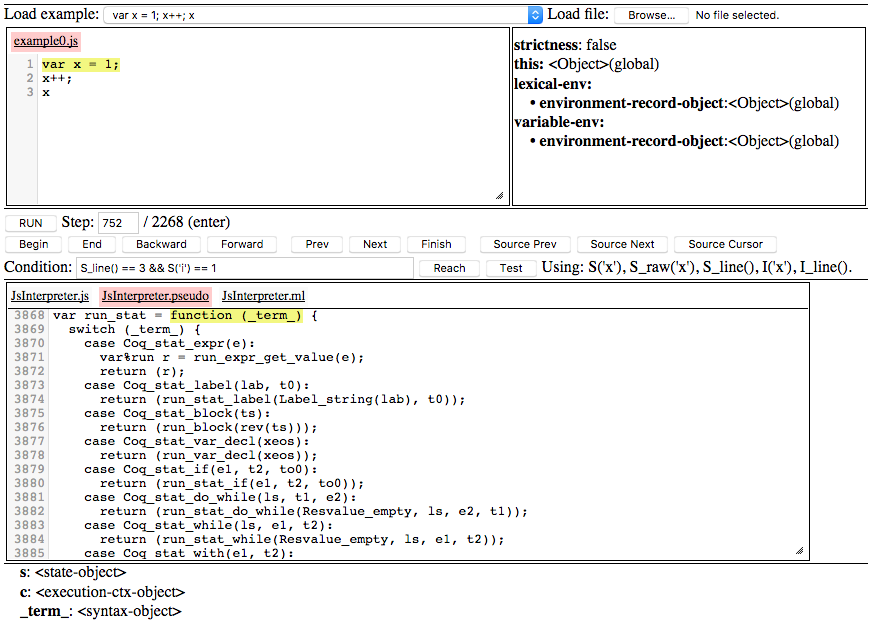
\includegraphics[width=\textwidth]{jsexplain.png}
  \caption{JSExplain}
  \label{fig:jsexplain}
\end{figure*}

JSExplain (Figure \ref{fig:jsexplain}) se présente sous la forme d'une
application web se composant principalement d'un interpréteur de Javascript
(dont le code est visible en bas de la figure) et d'une interface permettant
d'écrire du code (en haut à gauche). L'état du programme interprété est visible
en haut à droite, et l'état de l'interpréteur tout en bas. La zone centrale permet
de naviguer dans l'exécution du programme.

L'exécution du programme n'est pas directement interactive : le programme est
exécuté en entier lorsque le bouton \texttt{run} est appuyé, et son exécution
génère une trace qui peut ensuite être naviguée en utilisant l'interface.

Le code de l'interpréteur est annoté avec des instructions permettant de générer
ces traces lorsqu'il interprète un programme. Ces traces contiennent l'état de
l'interpréteur au moment de leur génération, ainsi que le contexte d'exécution
du programme interprété. Elles sont générées grâce à des appels à la fonction de
log \verb|log_event|. Dans l'exemple de la figure \ref{log_event}, une trace est
générée pour signaler une instruction de retour de fonction. La valeur de retour
est sauvegardée (la variable \verb|_return_2|) ainsi que le contexte d'exécution
(la variable \verb|ctx_1|). Les contextes sont implémentés par un encodage des
listes dans des objets JavaScript.
\begin{figure}[ht]
\begin{minted}{javascript}
log_event("MLInterpreter.js",
  1,
  ctx_push(ctx_1, [{key: "#RETURN_VALUE#", val:_return_2}]),
  "return");
\end{minted}
\caption{Appel à log\_event extrait de MLInterpreter.log.js}
\label{log_event}
\end{figure}

L'interpréteur de JSExplain, ainsi que celui de MLExplain, sont écrits en OCaml
et non pas directement en JavaScript. Plus précisément, nous utilisons un
sous-ensemble de OCaml, que nous appelons fOCaml, qui est purement fonctionnel
et décrit en détails ci-dessous. Le code fOCaml est compilé vers fJS, un sous
ensemble fonctionnel de JavaScript, grâce à un compilateur préservant autant que
possible la structure du code. Ce compilateur sert également à intégrer les
appels à \verb|log_event| lorsque le fichier est compilé en mode \emph{log}. La
figure \ref{arch_jsexplain} décrit ce fonctionnement. Le mode \emph{unlog} de ce
compilateur permet de compiler le code OCaml vers du Javascript sans
annotations. Le but de ce mode de compilation est de pouvoir ignorer une partie
du code de l'interpréteur lors de la génération des traces. Grâce à cela,
l'affichage des traces d'exécution ne sera pas pollué par des détails
d'implémentation de fonctions annexes.

\begin{figure}[ht]
  \begin{center}
  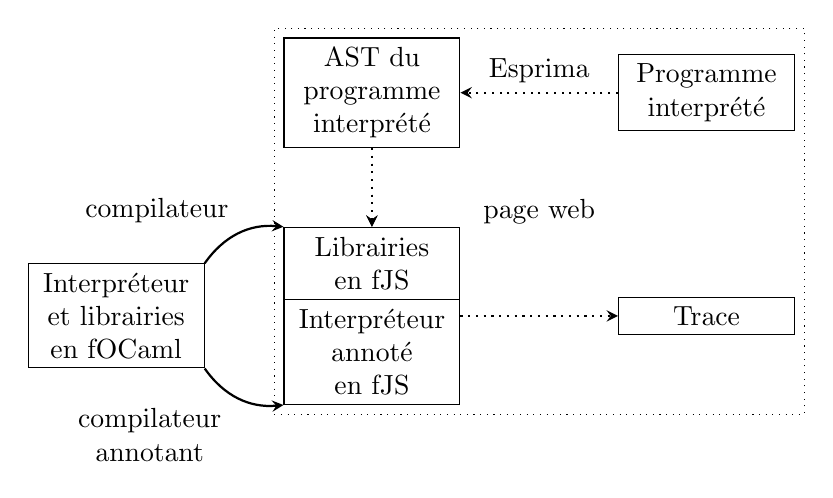
\begin{tikzpicture}[nodes = {align = center}]
    \node (focaml) [draw, text width=2cm] {Interpréteur et librairies en fOCaml};
    \node (fjs) [draw, right = 1cm of focaml, text width=2cm, rectangle split, rectangle split parts=2, text centered] 
{Librairies en fJS \nodepart{second} Interpréteur annoté en fJS};
    \node (ast) [draw, above = of fjs, text width=2cm] {AST du programme interprété};
    \node (source) [draw, right = 2cm of ast, text width=2cm, text centered] 
{Programme interprété};
    \node [draw, dotted, fit=(fjs) (ast) (source)] {page web};
    \node (trace) [draw, right = 2cm of fjs, text width=2cm, text centered] 
{Trace};
    \path[->,thick,>=stealth] (focaml.north east) edge[bend left] node[above left] {compilateur} (fjs.north west) ;
    \path[->,thick,>=stealth] (focaml.south east) edge[bend right] node[below left] {\parbox{2cm}{\centering compilateur annotant}} (fjs.south west);
    \path[->,thick,dotted,>=stealth] (source) edge node [above] {Esprima} (ast);
    \path[->,thick,dotted,>=stealth] (ast) edge (fjs);
    \path[->,thick,dotted,>=stealth] (ast) edge (fjs);
    \path[->,thick,dotted,>=stealth] (fjs) edge (trace);
  \end{tikzpicture}
  \end{center}
  
  \caption{Architecture de JSExplain}
  \label{arch_jsexplain}
\end{figure}

Le compilateur utilisé par JSExplain afin de générer du Javascript annoté ne 
reconnaît pas tout le langage OCaml mais un sous-ensemble de ce dernier. Cette 
limitation vient du fait que compiler de l'OCaml vers du JavaScript n'est pas 
trivial. De nombreuses fonctionnalités avancées, comme les motifs imbriqués, 
sont difficiles à représenter en JavaScript, c'est la raison pour laquelle ce 
compilateur ne gère qu'un sous-ensemble simple d'OCaml qui peut se compiler de 
manière quasi-transparente en JavaScript. À cause de cela, il est nécessaire 
d'adapter sa façon d'écrire, ce qui peut donner du code long et fastidieux.

\asi{dire que utilisions initialement une implémentation en JavaScript des
  tableaux semi-persistants \cite{DBLP:conf/esop/ConchonF08} pour représenter la
  mémoire JavaScript, mais nous avons depuis réimplémenté et étendu le module
  Map dans notre sous-ensemble de OCaml.}

L'interface web de JSExplain est une page HTML pouvant être découpée en trois
parties. La première partie est une zone de texte où l'utilisateur peut écrire
du code Javascript afin que celui-ci soit interprété. La seconde partie, à
droite de la première, est un cadre dans lequel état du programme précédemment
écrit est détaillé. Dans cet encadré sera affiché le contexte d'exécution ainsi
que la valeur des différentes variables définies dans le code. Enfin, la
troisième partie de cette page, en bas de la première, détaille l'état de
l'interpréteur. Le code de l'interpréteur, lui aussi affiché sur cette partie, 
défile en fonction de l'instruction en cours d'exécution. Cette instruction est 
surlignée afin d'être mise en évidence.

\subsection{OCaml}
Caml est un langage fonctionnel de la famille des langages ML développé par 
l'Inria. Objective Caml (ou OCaml) en est l'implémentation de référence. OCaml 
est utilisé dans des projets divers comme l'outil de développement web Ocsigen 
ou l'assistant de preuves interactif Coq. OCaml est un langage adapté à 
l'écriture de compilateurs, c'est la raison pour laquelle il est utilisé dans ce 
projet.

La grande majorité du code OCaml écrit dans JSExplain ne représente qu'un 
sous-ensemble du langage. En effet, l'un des compilateurs utilisés et présenté 
dans la section suivante ne gère qu'une sous-ensemble très restraint du langage 
OCaml. Il n'est pas possible d'utiliser les fonctionalités impératives et 
objets du langage et la bibliothèque standard est réduite à quelques fonctions 
du module \verb|Pervasives|. Par ailleurs, les motifs imbriqués ne sont pas 
disponibles non plus. Dans l'exemple suivant, \verb|Some 5| est un motif 
imbriqué puisqu'il s'agit d'un motif constructeur avec un motif constante en 
paramètre.

\begin{verbatim}
match x with
| Some 5 -> true
| None -> false
\end{verbatim}

Le seul moyen de travailler avec des motifs complexes est de lier les données à 
une variable et d'effectuer un filtrage supplémentaire :

\begin{verbatim}
match x with
| Some v ->
  begin
    match v with
    | 5 -> true
      | _ -> false
  end
| None -> None
\end{verbatim}

\section{Liste des technologies utilisées}
MLExplain est un projet complexe réunissant plusieurs langages. Dans cette 
partie nous présenterons ces langages ainsi que les principaux outils utilisés 
pour mettre au point MLExplain.

\section{Langages utilisés}
\subsection{Javascript}
Javascript est un langage de script orienté objet à prototypes. Il est 
principalement employé dans le développement de pages web interactives, mais 
aussi dans des applications serveurs grâce à des plateformes de développement 
telles que NodeJS.

MLExplain utilise intensivement javascript comme langage cible, puisque 
l'interpréteur d'OCaml est entièrement compilé vers javascript. Il est aussi 
utilisé pour manipuler l'interface web de MLExplain.



\section{Fonctionnement de JSExplain}
JSExplain est un interpréteur visuel pour javascript. C'est à dire un 
interpréteur capable d'afficher l'état du programme exécuté ainsi que son 
propre état au fur et à mesure de l'exécution. Pour que l'interpréteur puisse 
afficher l'état dans lequel il se trouve, il est compilé grâce à un compilateur 
qui ajoute des appels à une fonction de traçage. Les traces obtenues au fur et 
à mesure de l'exécution permettent de savoir, à tout moment, quelles variables 
existent, leur valeur ainsi que les valeurs de retour des fonctions de 
l'interpréteur. L'interface peut réutiliser ces traces afin de d'afficher 
l'état du programme et de l'interpréteur à chaque état de l'exécution.

\section{Architecture du code}
Dans ce chapitre nous traiterons de l'architecture du code de MLExplain. Nous 
allons expliquer le fonctionnement de l'application et nous expliquerons les 
différentes parties qui la composent. Par la suite nous détaillerons le code de 
l'interpréteur d'OCaml, qui est la partie centrale du projet.

\section{Compilation de code OCaml vers Javascript}
MLExplain étant une application web, elle nécessite la compilation du projet en 
javascript. Par ailleurs, le code de l'interpréteur OCaml est tracé grâce à un 
système d'enregistrement des évènements (appels de fonctions, retour de 
fonctions, définitions de variables...). Pour cela, nous utilisons deux 
compilateurs : js\_of\_ocaml et le compilateur de JSExplain.

\subsection{Le compilateur de JSExplain}
Le projet JSExplain, sur lequel est basé MLExplain, utilise son propre 
compilateur d'OCaml. Le but de ce compilateur est d'être capable de placer des 
appels à la fonction \verb|log_event| qui sert à tracer l'état de l'interpréteur 
au fur et à mesure de son exécution. Il sert aussi à récupérer les emplacements 
des différents objets syntaxiques dans le fichier source afin de produire le 
surlignage du code dans l'interface de JSExplain.

Ce compilateur propose plusieurs modes de fonctionnement :

\begin{itemize}
 \item unlog : génère un fichier javascript sans traçage
 \item log : génère un fichier javascript dans lequel les fonctions sont tracées
 \item mlloc, token et ptoken : génèrent des fichiers contenant des informations
sur le placement des éléments syntaxiques du fichier de départ.
 \item pseudo : génère un fichier de pseudo javascript amélioré avec du sucre 
syntaxique pour les opérations de filtrage et les opérations monadiques.
\end{itemize}

Seul le fichier \emph{MLInterpreter.ml} dans le dossier \emph{mlexplain} est 
tracé, puisqu'il contient les algorithmes pour l'interprétation de code OCaml.

\paragraph{Utilisation de monades}
Puisque le compilateur de JSExplain supporte un sous-ensemble limité d'OCaml, 
nous n'avons pas pu utiliser certaines fonctionalités très communes du langage 
telles que les exceptions. C'est la raison pour laquelle nous avons eu recours 
à des constructions comme les monades.

Une monade est une structure de donnée qui représente une action dans un 
contexte. Elles prennent la forme d'un constructeur de type. Les monades 
mettent à disposition les fonctions suivantes :

\begin{verbatim}
 Soit une monade m :
 
 val return : 'a -> 'a m
 val (>>=) : 'a m -> ('a -> 'b m) -> 'b m
\end{verbatim}

La fonction \verb|return| (ou \verb|unit|) permet de contruire une valeur 
monadique \verb|'a M| à partir d'une valeur de type \verb|'a|. Cette fonction 
permet d'injecter une valeur dans une monade.

La fonction \verb|bind| (ou l'opérateur infixe \verb|>>=|) sert à composer des 
monades à l'aide d'une fonction de type \verb|'a -> 'b m|.

% blablabla

Les monades obéissent aux lois suivantes :

\begin{align*}
m \Rightarrow return &\equiv m && \text{return est l'élément neutre de bind} \\
(\textit{\mbox{return x}}) \Rightarrow f &\equiv f(x) && \text{composition à 
gauche} \\
(m \Rightarrow f) \Rightarrow g &\equiv m \Rightarrow (x \mapsto f(x) 
\Rightarrow g) && \text{associativité}
\end{align*}
Le symbole $\Rightarrow$ correspond à l'opérateur \verb|>>=|.

Comme dit précédemment, les monades sont utilisées afin de calculer dans un 
contexte. Dans le cadre de MLExplain, elles permettent de gérer élégamment les 
erreurs. Nous utilisons le type \verb|Unsafe.t| défini ainsi :

\begin{verbatim}
type ('a, 'b) t =
| Error of string (* Erreur de l'interpréteur *)
| Except of 'a (* Exception dans le programme interprété *)
| Result of 'b (* Résultat dans le programme interprété *)
\end{verbatim}

% A partir de là un peu hors-sujet et pas nécessairement pertinent
Le constructeur \verb|Result| correspond à un calcul réussi tandis que les deux 
autres constructeurs correspondent à une erreur. Une fonction susceptible 
d'échouer retournera un \verb|Unsafe.t|. Par exemple, une division pourrait 
s'écrire ainsi :

\begin{verbatim}
let div : int -> int -> (string, int) Unsafe.t =
  fun a -> function
  | 0 -> Unsafe.Except "Division by zero"
  | b -> Unsafe.Result (a / b)
\end{verbatim}

Dans le code précédent, on voit que \verb|div x| est de type \verb|int -> (string, int) Unsafe.t|,
ce qui correspond parfaitement au type de la fonction dont \verb|>>=| a besoin. On pourrait alors écrire :

\begin{verbatim}
let res = Unsafe.Result 5 >>= div 3 in
match res with
| Unsafe.Error err -> prerr_endline err
| Unsafe.Except err -> prerr_endline err
| Unsafe.Result r -> print_int r
\end{verbatim}

Grâce à cette construction, il nous est possible de chaîner les \verb|bind| et 
ainsi de composer nos monades pour protéger tout un algorithme de l'échec. Nous 
avons utilisé une extension de syntaxe afin de rendre cette chaîne de 
\verb|bind| plus lisible :

\begin{verbatim}
let%result a = Unsafe.Result 5 in
div 3 a

(* équivaut à *)
Unsafe.Result 5 >>= div 3
\end{verbatim}	

\subsection{Le compilateur js\_of\_ocaml}
Le compilateur js\_of\_ocaml est un compilateur de bytecode OCaml vers 
javascript créé par l'Université Paris-Diderot et Be Sport. Nous utilisons ce 
compilateur afin de générer le javascript pour la partie frontale de notre 
interpréteur. Le compilateur de JSExplain ne permet pas d'utiliser des paquets 
externes, ce qui nous pousse à utiliser un autre compilateur. En effet l'analyse 
lexicale et syntaxique ainsi que le typage dans notre interpréteur sont gérés 
grâce au paquet \emph{compiler-libs} d'OCaml. De plus, la partie frontale de 
l'interpréteur ne doit pas être tracée, il n'est donc pas nécessaire d'utiliser 
le compilateur de JSExplain.

L'utilisation d'un autre compilateur nous pousse à devoir convertir l'AST du 
programme en javascript explicitement afin que sa représentation en mémoire 
soit la même que celle attendue par le code compilé par le compilateur de 
JSExplain.

\section{L'interpréteur d'OCaml}

\begin{figure}[ht]
  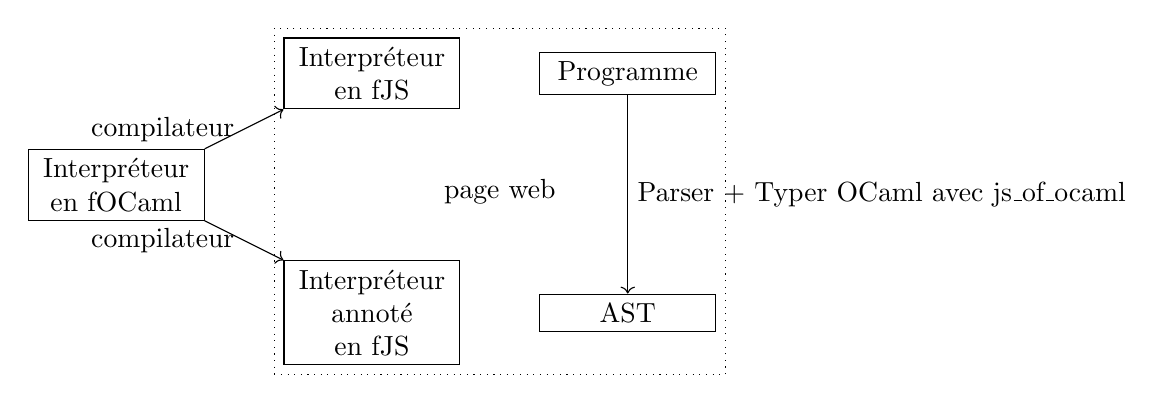
\begin{tikzpicture}[nodes = {align = center}]
    \node (focaml) [draw, text width=2cm] {Interpréteur en fOCaml};
    \node (fjs) [draw, above right = 0.5cm and 1cm of focaml, text width=2cm] 
{Interpréteur en fJS};
    \node (fjsa) [draw, below right = 0.5cm and 1cm of focaml, text width=2cm] 
{Interpréteur annoté en fJS};
    \node (ast) [draw, right = of fjsa, text width=2cm] {AST};
    \node (source) [draw, right = of fjs, text width=2cm, text centered] 
{Programme};
    \node [draw, dotted, fit=(fjs) (fjsa) (ast)] {page web};
    \draw[->] (focaml.north east) -- node[left] {compilateur} (fjs.south west) ;
    \draw[->] (focaml.south east) -- node[left] {compilateur} (fjsa.north west);
    \draw[->] (source) -- node [right] {Parser + Typer OCaml avec js\_of\_ocaml} (ast);
  \end{tikzpicture}
  
  \caption{Architecture de MLExplain}
  \label{arch_mlexplain}
\end{figure}

\asi{Je propose de ne parler que de MLExplain et pas de l'autre interpréteur.}

Deux versions de l'interpréteur ont été écrites. La première version est 
compilée vers javascript afin d'être intégrée à l'interface web de MLExplain. 
Elle se base sur l'arbre syntaxique abstrait typé d'OCaml (le \emph{Typedtree}).
La seconde version est un interpréteur interactif en ligne de commande écrit
en OCaml et compilé avec le compilateur standard du langage. Cet interpréteur 
se base sur l'arbre syntaxique abstrait non typé d'OCaml dans le but de réduire 
au maximum la dépendence envers le compilateur officiel et se limiter à 
l'analyseur syntaxique. L'interpréteur en ligne de commande exécute donc du code
OCaml non typé.

Ne pas typer le code OCaml a été une source de problème majeure. Certaines 
fonctionnalités du langage telles que les paramètres nommés et optionnels des 
fonctions ne peuvent pas être interprétées sans un typage préalable du code.

\subsection{Arichtecture du code}
L'ensemble des sources de l'interpréteur d'OCaml se trouve dans le dossier 
\emph{mlexplain/} et peut se découper en trois parties : la partie 
frontale, la gestion de l'état et des contextes des programmes et enfin 
l'exécution du code.

La partie frontale de l'interpréteur se trouve essentiellement dans le fichier 
\emph{TranslateSyntax.ml}. Ce fichier se charge de la traduction de 
l'arbre syntaxique typée construit par la compiler-libs vers l'arbre de syntaxe 
défini dans \emph{MLSyntax.ml} puis de la traduction de cet arbre vers son 
équivalent javascript. Puisque la partie frontale de l'interpréteur n'est pas 
compilée avec le même compilateur que le reste du code, il est nécessaire de 
traduire explicitement l'AST vers javascript pour obtenir la même 
représentation interne que celle attendue par la partie arrière de 
l'interpréteur. C'est aussi dans le fichier \emph{TranslateSyntax.ml} que se 
trouve la définition de l'objet javascript \verb|MLExplain| contenant les 
méthodes \verb|parseExpr| et \verb|parseStructure| appelées depuis l'interface 
de JSExplain.

Le compilateur OCaml vers javascript de JSExplain ne permet pas d'utiliser la 
bibliothèque standard d'OCaml, c'est la raison pour laquelle plusieurs modules 
auxiliaires ont été développés au sein de MLExplain. Parmi ces modules, les 
plus importants sont \verb|MLArray|, \verb|MLList|, \verb|Vector| et 
\verb|Map|.

\verb|MLArray| et \verb|MLList| implémentent une partie des fonctions de la 
bibliothèque standard, ainsi que quelques fonctions utiles, permettant 
d'utiliser des listes et tableaux en OCaml. \verb|Vector| implémente un type 
\verb|'a vec| représentant un tableau muable dynamique (un vecteur). Ce module 
est écrit en javascript, puisqu'il n'est pas possible de le faire avec le 
sous-ensemble d'OCaml géré par le compilateur de JSExplain. Ce module sert à 
modéliser l'état du programme exécuté, à chaque indice du vecteur est associé 
une valeur et donc, chaque indice sert de référence vers cette valeur. Le 
module \verb|Map| permet l'utilisation de listes associatives. Ces listes sont 
utilisé dans MLExplain pour gérer les contextes d'exécution. À chaque 
identifiant est associé un indice dans le vecteur état du programme.

La partie arrière de l'interpréteur comprend les modules \verb|Value| et 
\verb|MLInterpreter|. Le module \verb|Value| définit le type \verb|value| qui 
modélise les données OCaml ainsi que des fonctions qui permettent de manipuler 
des \verb|value|, notamment le test d'égalité. Le module \verb|MLInterpreter| 
contient les algorithmes d'exécution du code.
\bibliographystyle{plain}
\bibliography{jfla}

\end{document}

%%% Local Variables:
%%% coding: utf-8
%%% mode: latex
%%% TeX-engine: latex_sh
%%% End: